\subsection{Selección y modelado de estilos y patrones}

Los estilos arquitectónicos guían la composición y relación de los componentes en un sistema de software. A continuación, se presentan brevemente los estilos seleccionados para la implementación de la solución.

\textbf{Estilo Llamada-Retorno}

El sistema sigue un enfoque de "Llamada-Retorno", donde las capas del sistema se comunican a través de llamadas y retornos de resultados. Esto se aplica a la interacción entre la capa de presentación, la capa de lógica de negocio y la capa de acceso a datos (\autoref{fig:call-return-style}), asegurando una separación clara de responsabilidades y facilitando la escalabilidad y mantenibilidad del software.

En la \autoref{fig:call-return-style-example} se muestra un ejemplo de puesta en práctica de este estilo en el sistema, donde la capa de lógica de negocio \underline{llama} a la función \textbf{getDirectChildren} de de la capa de acceso a datos, la cual \underline{retorna} los hijos directos de una entrada  del directorio.

\begin{figure}[th]
    \centering
    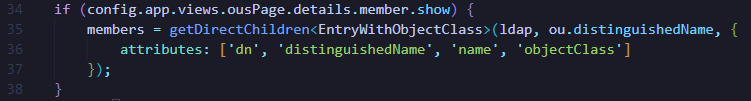
\includegraphics[width=\linewidth]{images/code/getDirectChildren-call.png}
    \caption{Ejemplo del estilo Llamada-Retorno en el sistema}
    \label{fig:call-return-style-example}
\end{figure}

\textbf{Patrón Cliente-Servidor}

El sistema implementa el patrón Cliente-Servidor, donde el cliente (la interfaz de usuario) se comunica con el servidor para solicitar servicios o datos. Este patrón facilita la separación de responsabilidades y la escalabilidad del sistema. Esta comunicación se realiza en su mayoría mediante el envío de formularios.

\textbf{Patrón de Acceso a Datos}

Para la gestión de los datos en el sistema, se implementa el Patrón de Acceso a Datos como un intermediario entre los servicios de la aplicación y el AD. Específicamente, este patrón facilita las siguientes operaciones:
\begin{itemize}
    \item \textbf{Abstracción del AD}: Se usa la librería ldapts, que abstrae las interacciones con el AD, simplificando el código y reduciendo errores.
    \item \textbf{Centralización de acceso}: Todas las solicitudes de datos pasan por esta capa, asegurando un flujo controlado y consistente.
    \item \textbf{Seguridad centralizada}: La capa implementa políticas de seguridad uniformes para todas las operaciones en el AD.
\end{itemize}

En la \autoref{fig:using-ldap-client-to-search-in-directory} muestra la declaración de la función \textbf{getDirectChildren} mencionada anteriormente, donde se utiliza el cliente ldap (de la librería ldapts) para realizar una búsqueda en el directorio. El uso del cliente ldap abstrae la interacción con el directorio además de centralizar el acceso.

\begin{figure}[h]
    \centering
    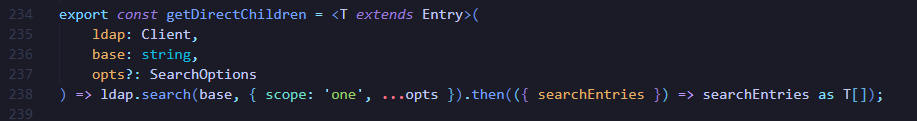
\includegraphics[width=\linewidth]{images/code/getDirectChildren.png}
    \caption{Uso del cliente ldap para realizar una búsqueda en el directorio}
    \label{fig:using-ldap-client-to-search-in-directory}
\end{figure}

\textbf{Patrón n-capas}
La arquitectura del sistema está organizada en un patrón de n-capas (\autoref{fig:n-layer-system-structure}), con una capa de presentación que interactúa con la capa de lógica de negocio, la cual a su vez se comunica con la capa de acceso a datos. Este enfoque modulariza las responsabilidades y mejora la escalabilidad y mantenibilidad del sistema.

\begin{figure}[h]
    \centering
    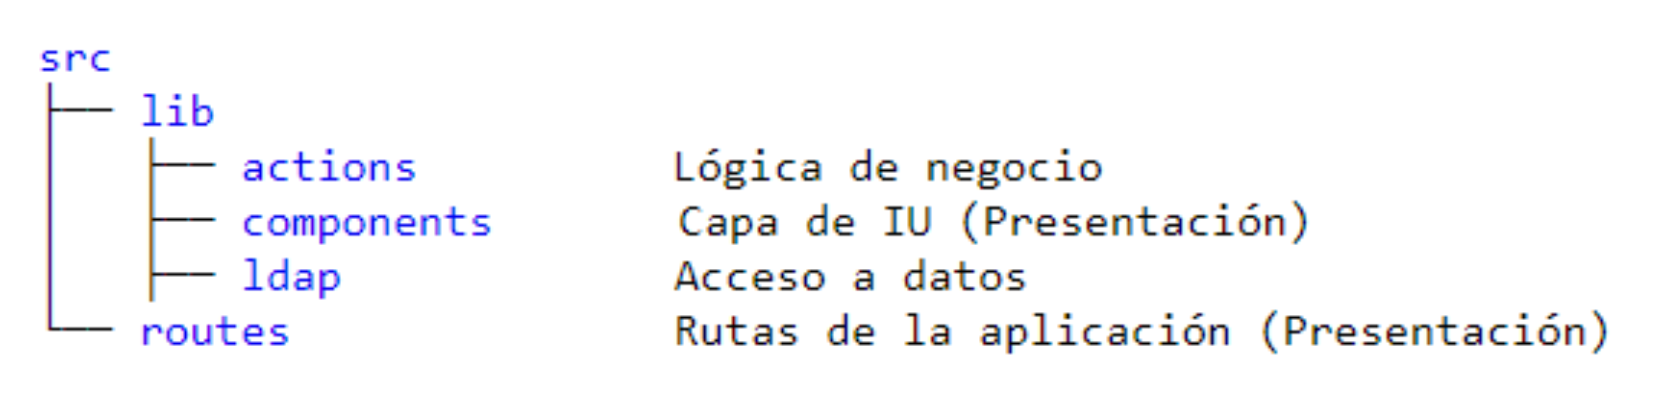
\includegraphics[width=\linewidth]{images/app-folder-structure.png}
    \caption{Estructura simplificada del sistema mostrando n-capas}
    \label{fig:n-layer-system-structure}
\end{figure}